%!TEX root = ../egpaper_for_review.tex

\newcounter{cX}
\newcounter{cY}


\newcounter{NPY}
\setcounter{NPY}{30}
\tikzstyle{pixel}=[opacity=1.0,thick,draw opacity=1.0, draw=black]
\tikzstyle{ln}=[opacity=0.6,fill=green,circle,draw, inner sep=0,font=\tiny,minimum size=0.15cm]
\tikzstyle{gn}=[opacity=0.6,fill=red,circle,draw, inner sep=0,font=\tiny,minimum size=0.15cm]
\tikzstyle{p}=[opacity=0.6,fill=white,circle,draw, inner sep=0,font=\tiny,minimum size=0.15cm]
\begin{figure}[H]
\begin{center}
\begin{tikzpicture}[scale=1.0]
    \node[anchor=south west,inner sep=0] (image) at (0,0) 
        {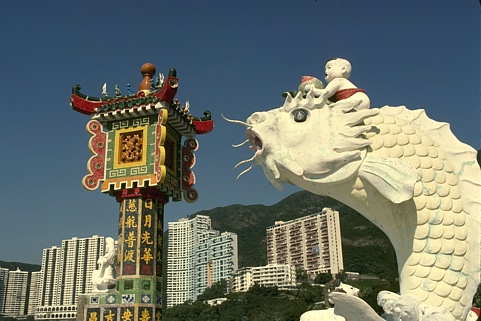
\includegraphics[width=0.4\textwidth]{images/120093.jpg}};
    % shift scope to the image 
    \begin{scope}[x={(image.south east)},y={(image.north west)},xscale=100/481,yscale=100/321]   
        \draw[gray,xstep=3.21/\theNPY, ystep=3.21/\theNPY] (0,0) grid (4.81,3.21);
        % scope of the grid
        \begin{scope}[xscale=3.21/\theNPY,yscale=3.21/\theNPY]  

        \foreach \x\y in {22/18, 10/8} { 
        \setcounter{cX}{\x}
        \setcounter{cY}{\y}
        \draw (\thecX+0.5,\thecY+0.5) node[p]  (centerPixel){};
        \foreach \xx in {-4,0,4} { 
        \foreach \yy in {-4,0,4} { 
            \ifthenelse{\NOT 0 = \xx \OR \NOT 0 = \yy}{
                %\filldraw[green!40!white,pixel] 
                %(\thecX+\xx,\thecY+\yy) rectangle (\thecX+1+\xx,\thecY+1+\yy);
                \draw (\thecX+\xx+0.5,\thecY+\yy+0.5) node[gn](nonLocalPixel){};
                \path[]
                (centerPixel) edge[bend left=0*\xx*\yy ] (nonLocalPixel)
                ;
            }{
            }
        }
        }
        \foreach \xx/\yy/\pColor in {0/1/blue, 0/-1/blue, 1/0/blue, -1/0/blue} { 
            \draw (\thecX+\xx+0.5,\thecY+\yy+0.5) node[ln](nonLocalPixel){};
            (\thecX+\xx,\thecY+\yy) rectangle (\thecX+1+\xx,\thecY+1+\yy);
        }
        }
        % \filldraw[gray,pixel] (\thecX,\thecY) rectangle (\thecX+1,\thecY+1);
        

        \end{scope}
    \end{scope}


\end{tikzpicture}
\end{center}
\caption{
    Pixel Level Multicut:
    every pixel (white nodes) is connected
    to its 4 \emph{local} neighbors (edges between white and green nodes).
    Furthermore each pixel is connected to some \emph{non-local} neighbors within a 
    certain radius  (edges between white and green nodes).
    The local neighbors are connected with a \emph{positive}
    edge weight. If the edge indicator (as gradient magnitude)
    is very high, the local edge weight should be close to zero.
    If there is no evidence for a cut (low gradient magnitude for example)
    the local edge weight should be high.
    The \emph{non-local edge weights} are \emph{negative} to
    encourage label transitions.
    The weight of the non-local edge weights can
    be the negative value of the maximum gradient magnitude
    along a line between the red and white node.
    If there is evidence for a cut between red and white, 
    the weight should be strongly(?) negative.
}
\end{figure}




